\documentclass[a4paper,11pt,fleqn]{article}
%%%%% langues
\usepackage[french]{babel}

\usepackage{colortbl}
\usepackage[svgnames]{xcolor}

\definecolor{gris05}{gray}{0.95}

\usepackage{ifthen}

\newboolean{boolCom}
\newboolean{boolInd}
\newboolean{boolCor}

\setboolean{boolCom}{true}
\setboolean{boolInd}{true}
\setboolean{boolCor}{true}

\newcounter{cpt-activite}
\setcounter{cpt-activite}{0}

\newenvironment{Activite}[1]%
    {% 
       \addtocounter{cpt-activite}{1}  
       \setbox0=\hbox\bgroup% On met le contenu de la def dans une boîte
       \begin{minipage}{\textwidth}% On enrobe le tout dans un minipage
       \textbf{Activit\'{e}  \arabic{cpt-activite} #1}\\
      %
     }
     {%
       \end{minipage}
        \egroup% fin de la boîte
        \ifthenelse{\boolean{boolCom}}
        {
        \vspace{0.3cm}
        \noindent
          \fcolorbox{blue}{PaleTurquoise}{\box0}% On affiche la boîte avec un encadrement
        }
        {}
    }
 
 \newenvironment{Indication}[1]%
    {%   
       \setbox0=\hbox\bgroup% On met le contenu de la def dans une boîte
       \begin{minipage}{\textwidth}% On enrobe le tout dans un minipage
       \textbf{Indication \arabic{cpt-activite}}\\
      %
     }
     {%
       \end{minipage}
        \egroup% fin de la boîte
        \ifthenelse{\boolean{boolCom}}
        {
          \fcolorbox{Gold}{LightGoldenrodYellow}{\box0}% On affiche la boîte avec un encadrement
        }
        {}
    }
 \newenvironment{Corrige}%
    {%   
       \setbox0=\hbox\bgroup% On met le contenu de la def dans une boîte
       \begin{minipage}{\textwidth}% On enrobe le tout dans un minipage
       \textbf{\'El\'ements de solution \arabic{cpt-activite}}\\
      %
     }
     {%
       \end{minipage}
        \egroup% fin de la boîte
        \ifthenelse{\boolean{boolCor}}
        {
          \fcolorbox{DeepPink}{Pink}{\box0}% On affiche la boîte avec un encadrement
        }
        {}
    }
  

\usepackage{harvard}

\def\ftoday{\number\day\space
 \ifcase\month\or
janvier\or f{\'e}vrier\or mars\or avril\or mai\or juin\or
 juillet\or ao{\^u}t\or septembre\or octobre\or novembre\or d{\'e}cembre\fi
 \space\number\year}


%%%%% format de page 
 \setlength{\textwidth }{16cm} 
 \setlength{\oddsidemargin}{0cm} 
 \setlength{\evensidemargin}{0cm} 
 \setlength{\topmargin}{-1cm} 
 \setlength{\headheight}{1cm} 
 \setlength{\headsep}{0.5cm} 
 \setlength{\textheight}{24cm}
 

%\usepackage{draftwatermark}
%\SetWatermarkText{Document de travail}
%\SetWatermarkLightness{1}
%\SetWatermarkScale{0.5}

%%%%% Style de page
\newcommand\algorithme{Sciences Manuelles du Num\'{e}rique  \textit{Ghostbusters}}
\newcommand\site{}
\newcommand\etablissement{Universit{\'e} Joseph Fourier}
\newcommand\jour{version du \ftoday}
\usepackage{my-page}
\pagestyle{myheadings}

%%%%% fontes 
\usepackage[T1]{fontenc}
\usepackage[utf8]{inputenc}
\usepackage{times}


%%%%% algorithmes
\usepackage[french,vlined]{algorithm2e}

\SetKw{KwDownTo}{downto}
\SetKwIF{If}{ElseIf}{Else}{if}{}{else if}{else}{endif}
\SetKwFor{For}{for}{}{endfor}
\SetKwFor{While}{while}{}{endw}%

\SetKwInput{KwIn}{Entrée}%
\SetKwInput{KwOut}{Sortie}%
\SetKwInput{KwData}{Données}%
\SetKwInput{KwResult}{Résultat}%



 
 %%%%% boites
%\usepackage{psboxit}
\usepackage{fancybox}

%%%%% graphiques
\usepackage{pstricks,pst-plot,pst-text,pst-tree,pst-eps,pst-fill,pst-node,pst-math}

\usepackage{xcolor}
\usepackage{colortbl}
\usepackage{graphics}%
\usepackage{figlatex}%

\definecolor{gris05}{gray}{0.95}

%\graphicspath{{figures/}}%

%\usepackage{pgfplots}


%%%%% hyperliens
\usepackage{hyperref,url}
\hypersetup{
dvips,
backref=true, %permet d'ajouter des liens dans...
pagebackref=true,%...les bibliographies
hyperindex=true, %ajoute des liens dans les index.
colorlinks=true, %colorise les liens
breaklinks=true, %permet le retour à la ligne dans les liens trop longs
urlcolor= blue, %couleur des hyperliens
linkcolor= blue, %couleur des liens internes
bookmarks=true, %créé des signets pour Acrobat
bookmarksopen=true} 

%%%%%%%%% Listings
% Default fixed font does not support bold face
\DeclareFixedFont{\ttb}{T1}{txtt}{bx}{n}{12} % for bold
\DeclareFixedFont{\ttm}{T1}{txtt}{m}{n}{12}  % for normal

% Custom colors
\usepackage{color}
\definecolor{deepblue}{rgb}{0,0,0.5}
\definecolor{deepred}{rgb}{0.6,0,0}
\definecolor{deepgreen}{rgb}{0,0.5,0}

\usepackage{listings}

% Python style for highlighting
\newcommand\pythonstyle{\lstset{
language=Python,
basicstyle=\ttm,
otherkeywords={self},             % Add keywords here
keywordstyle=\ttb\color{deepblue},
emph={MyClass,__init__},          % Custom highlighting
emphstyle=\ttb\color{deepred},    % Custom highlighting style
stringstyle=\color{deepgreen},
frame=tb,                         % Any extra options here
showstringspaces=false            % 
}}


% Python environment
\lstnewenvironment{python}[1][]
{
\pythonstyle
\lstset{#1}
}
{}

% Python for external files
\newcommand\pythonexternal[1]{{
\pythonstyle
\lstinputlisting{#1}}}

% Python for inline
\newcommand\pythoninline[1]{{\pythonstyle\lstinline!#1!}}



%%%%% mathématiques
\usepackage{amsmath,amsfonts,amssymb,newlfont,latexsym}

% symboles
 \def\real{\mathbb{R}}
 \def\integer{\mathbb{N}}
 \def\relative{\mathbb{Z}}
 \def\Prob{\mathbb{P}}
 \def\Esp{\mathbb{E}}
 \def\1{\large{1\!\!1}}

\def\leq{\leqslant}%
\def\geq{\geqslant}%
 
 % expressions
 \def\limn{\lim_{ n \to +\infty}}
 \def\limt{\lim_{t \to +\infty}}

  % environnements
 \newtheorem{defi}{D{\'e}finition}
 \newtheorem{lemm}{Lemme}
 \newtheorem{prop}{Proposition}
 \newtheorem{coro}{Corollaire}
 \newtheorem{theo}{Th{\'e}or{\`e}me}
 \newtheorem{conj}{Conjecture}
%%%%%%%%%%%%%%%%%%%%%%%%%%%%%%%%%%%%%%%%%%%%%%%%%%%%%%%%%%%%%%%%%%%
\usepackage{float}
 
 
 
 % Definition generale des cadres
\newlength {\largeur}
\addtolength {\largeur}{\textwidth}
\addtolength {\largeur}{-4em}

\newenvironment{cadre}[1]%
  {% 

    \ \\
    \indent
    \begin{Sbox}%
      \begin{minipage}{\largeur}%
        \vspace{-0.5em}
        \hspace{-2ex}
        \colorbox{white}{\strut{\color{black}{\large \bf #1}\ \ }}\\
        \vspace{-0.7em}\ \\
        %\it
%        \vspace{-1.5em}\ \\
%        \colorbox{white}{\strut{\color{black}\ \ {\bf #1}\ \ }}\\
  }
  {\end{minipage}\end{Sbox}
\fboxsep 1em
\fbox{\TheSbox}\vspace{0em}\\
\fboxsep 0em
}

%\floatstyle{ruled}
\newfloat{my-algo}{thp}{lop}
\floatname{my-algo}{Algorithme}

\newcounter{cpt-question}
\newenvironment{question}[1]{\begin{description}\item [Question] 
                      \textbf{\addtocounter{cpt-question}{1}\arabic{cpt-question}}  #1
                      }{\end{description}}  
\setcounter{cpt-question}{0}  
           
\begin{document}
\thispagestyle{empty}

\vspace{-2cm}
\noindent
{\Large {Sciences Manuelles du Numérique \textit{Ghostbusters}} }\hfill 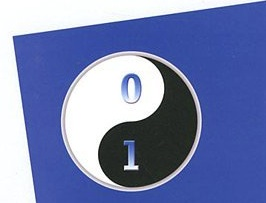
\includegraphics[width=1cm]{logos/isi2.jpg}

\noindent \hrulefill

\noindent
\textbf{}\\
\noindent
Auteur : Jean-Marc.Vincent@imag.fr\\
\noindent
\href{http://www.ujf-grenoble.fr/}{Université Grenoble-Alpes}, \href{http://ufrima.imag.fr/}{UFR IM$^\text{2}$AG},  \href{http://www.inria.fr/}{Inria Rhône-Alpes}, \href{http://www-irem.ujf-grenoble.fr/}{IREM-Grenoble}

\begin{quotation}
\textit{
There's something very important I forgot to tell you ! Don't cross the streams. . . It
would be bad. . .Try to imagine all life as you know it stopping instantaneously
and every molecule in your body exploding at the speed of light.}
Dr. Egon Spengler
\end{quotation}
Les chasseurs de fantômes Ghostbusters utilisent des rayons pour neutraliser les fantômes.
Comme l'indique la citation ci-dessus, il est primordial que ces rayons ne se croisent jamais.
Imaginons dix fantômes chassés par dix Ghostbusters. Ces derniers peuvent-ils se répartir
les fantômes afin que chacun tire sur un fantôme sans qu'aucun rayon ne se croise. \footnote{Merci à Romain Joly et Math en Jeans}
\begin{center}
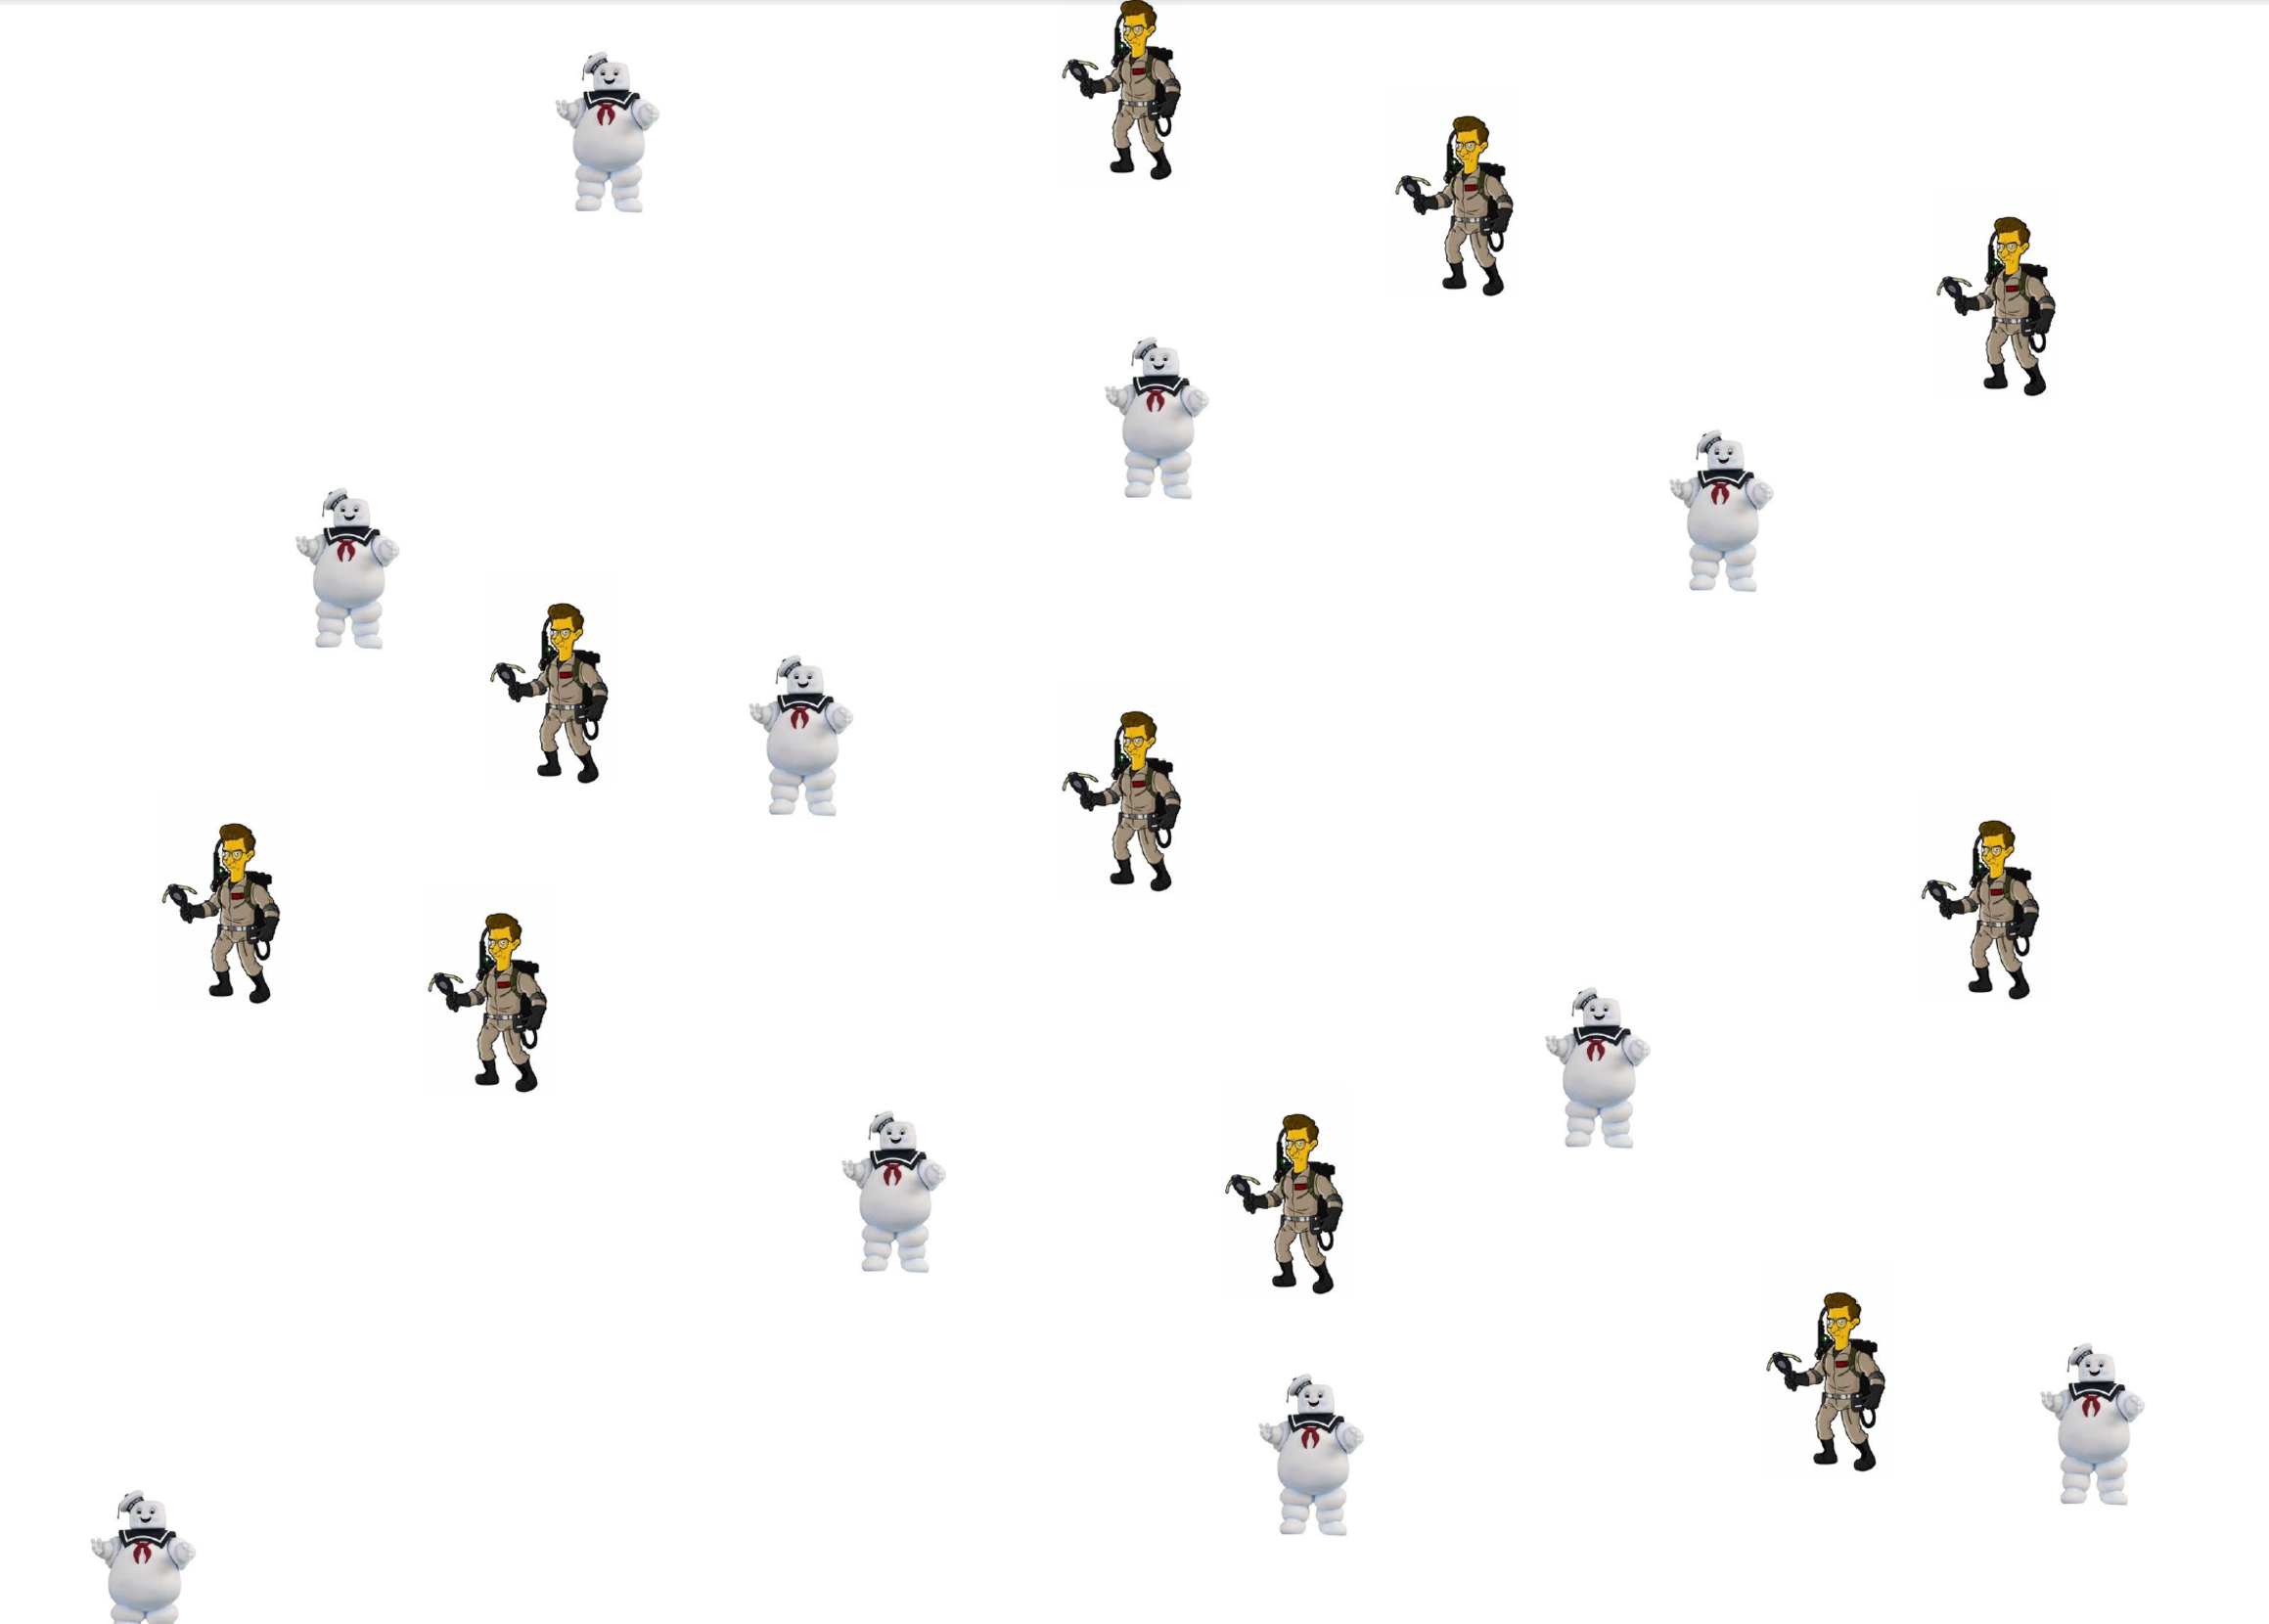
\includegraphics[width=0.4\linewidth]{figures/ghostbusters.pdf}
\end{center}
%On suppose que les positions des ghostbusters et des fantômes sont quelconques, c'est à dire que 3 d'entre eux ne sont jamais alignés. 

%% ici photo de la plaque
\begin{minipage}{0.3\linewidth}
%
\begin{center}
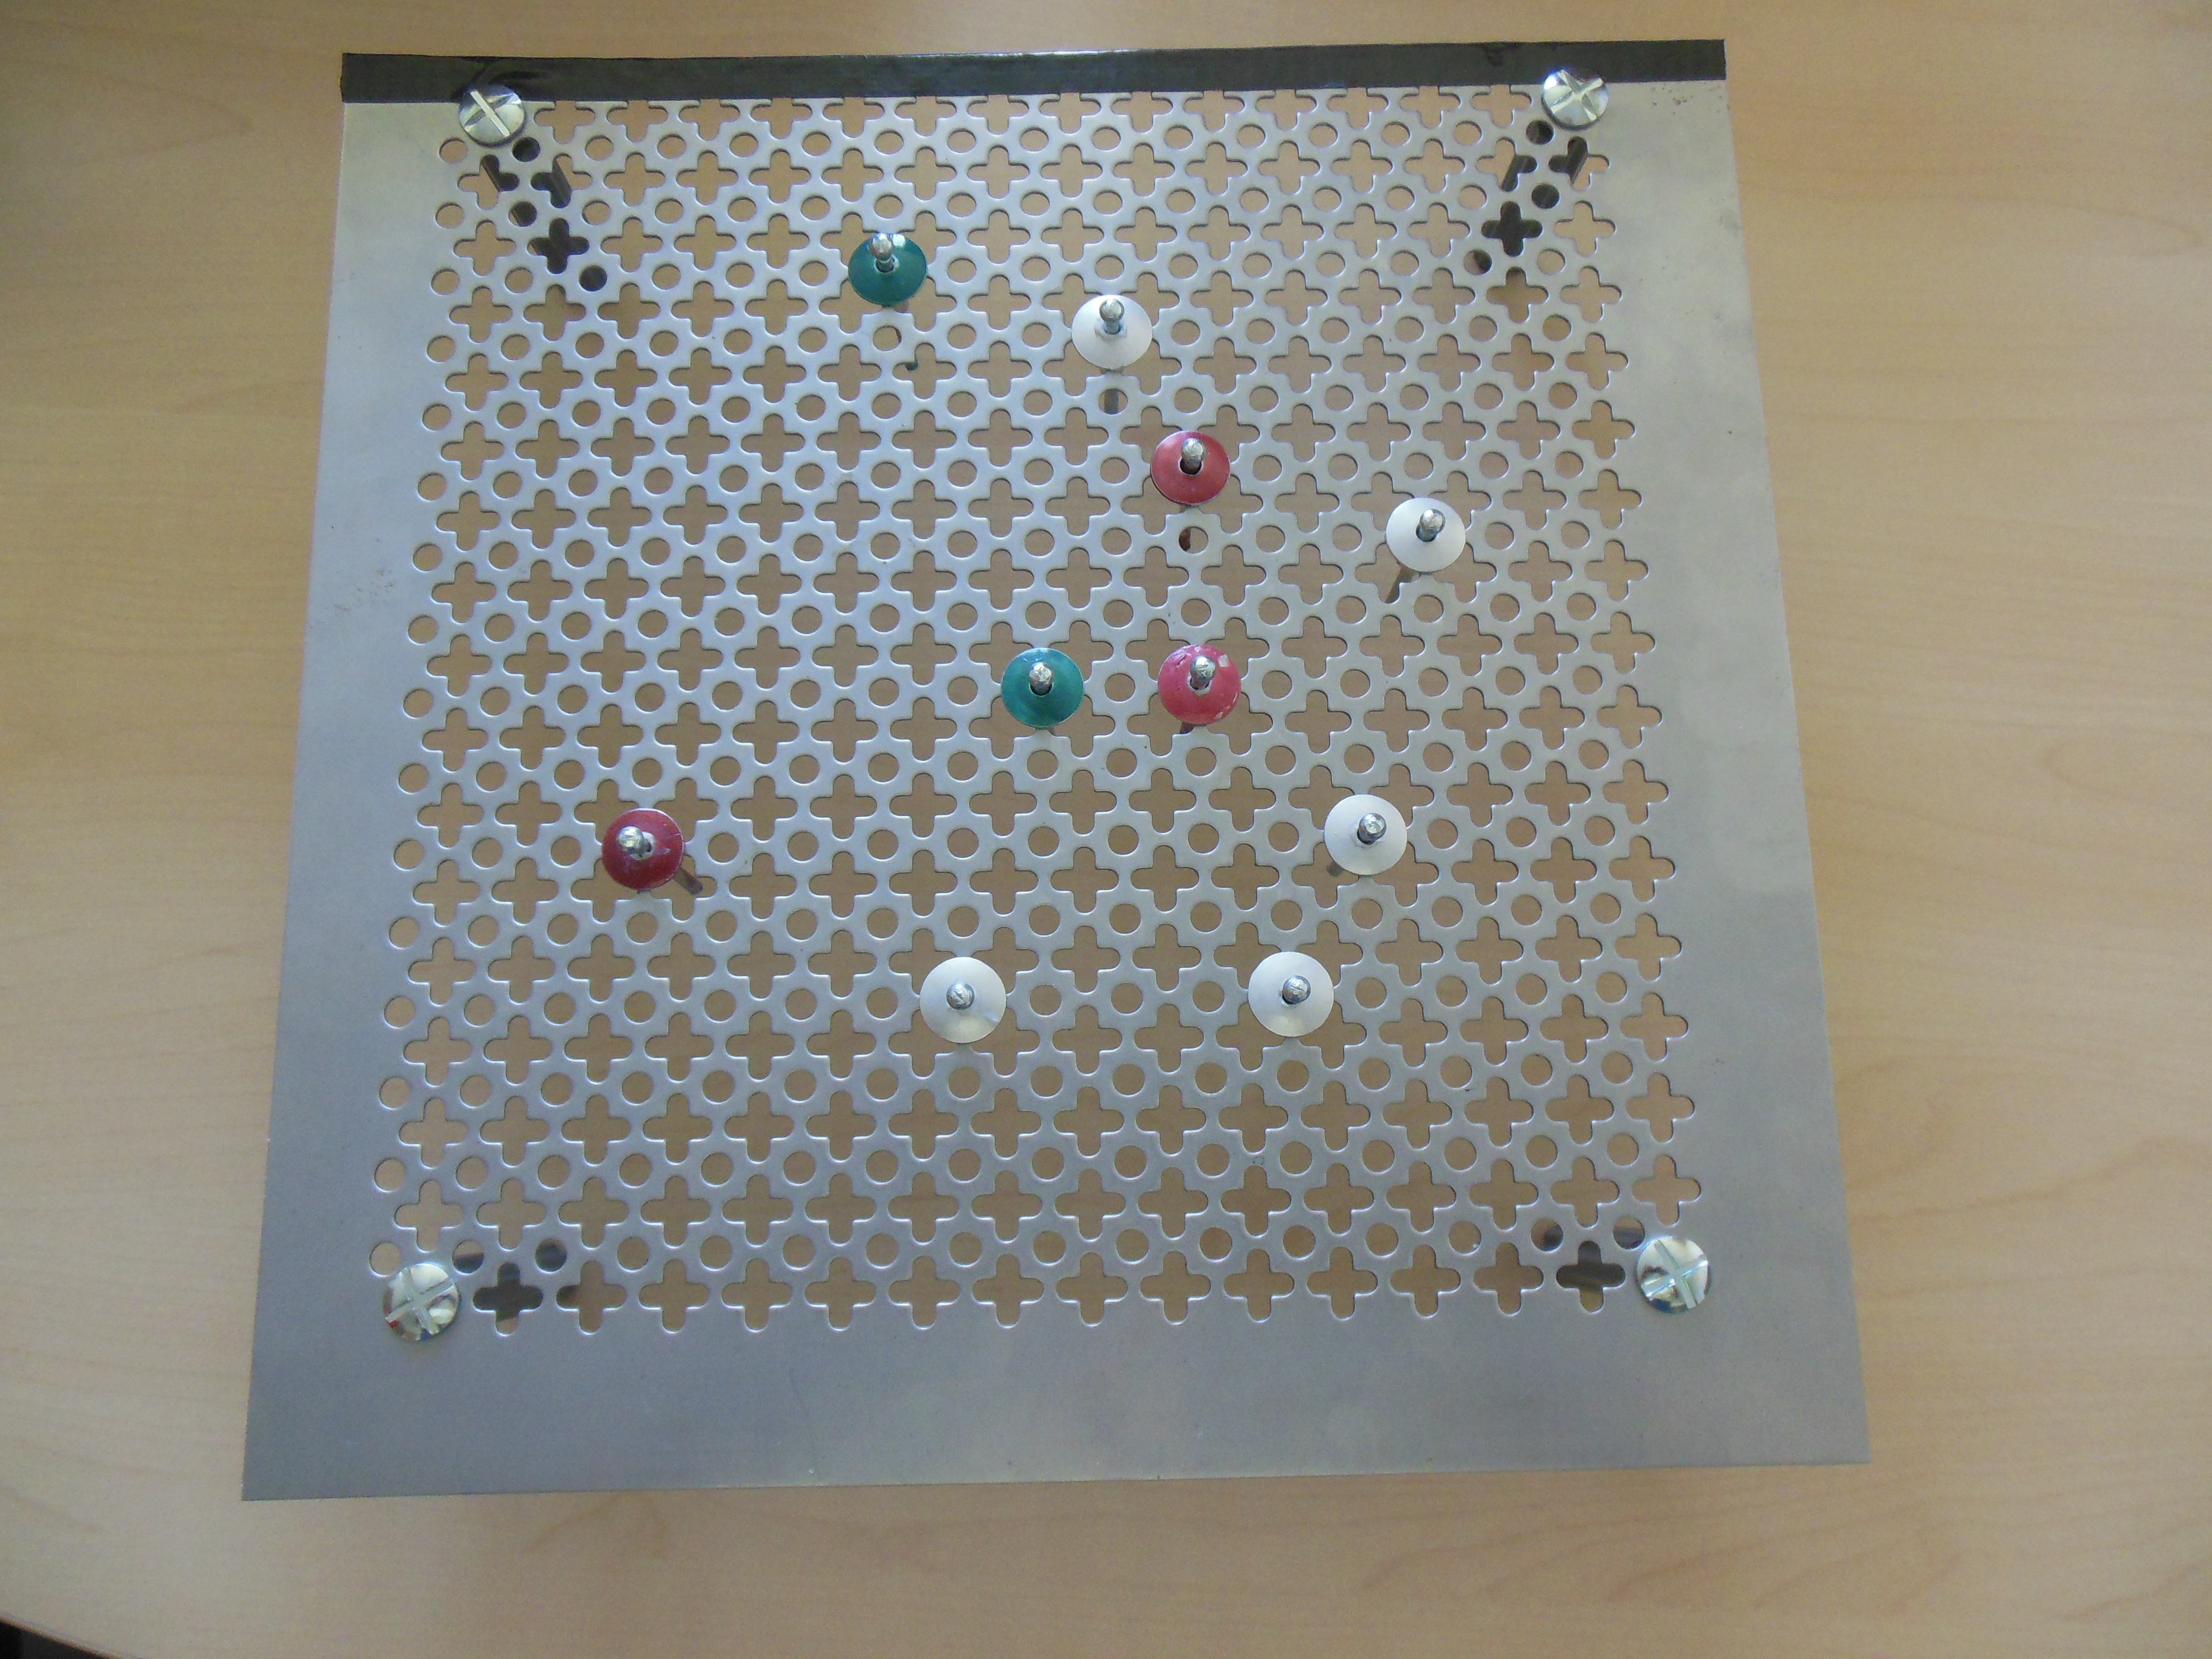
\includegraphics[width=\linewidth]{Photos/Ghosbusters-clous.pdf}
\end{center}
Ronds blancs : chasseurs, \\
Ronds colorés : fantômes.
\end{minipage}\hfill
\begin{minipage}{0.3\linewidth}

\begin{center}
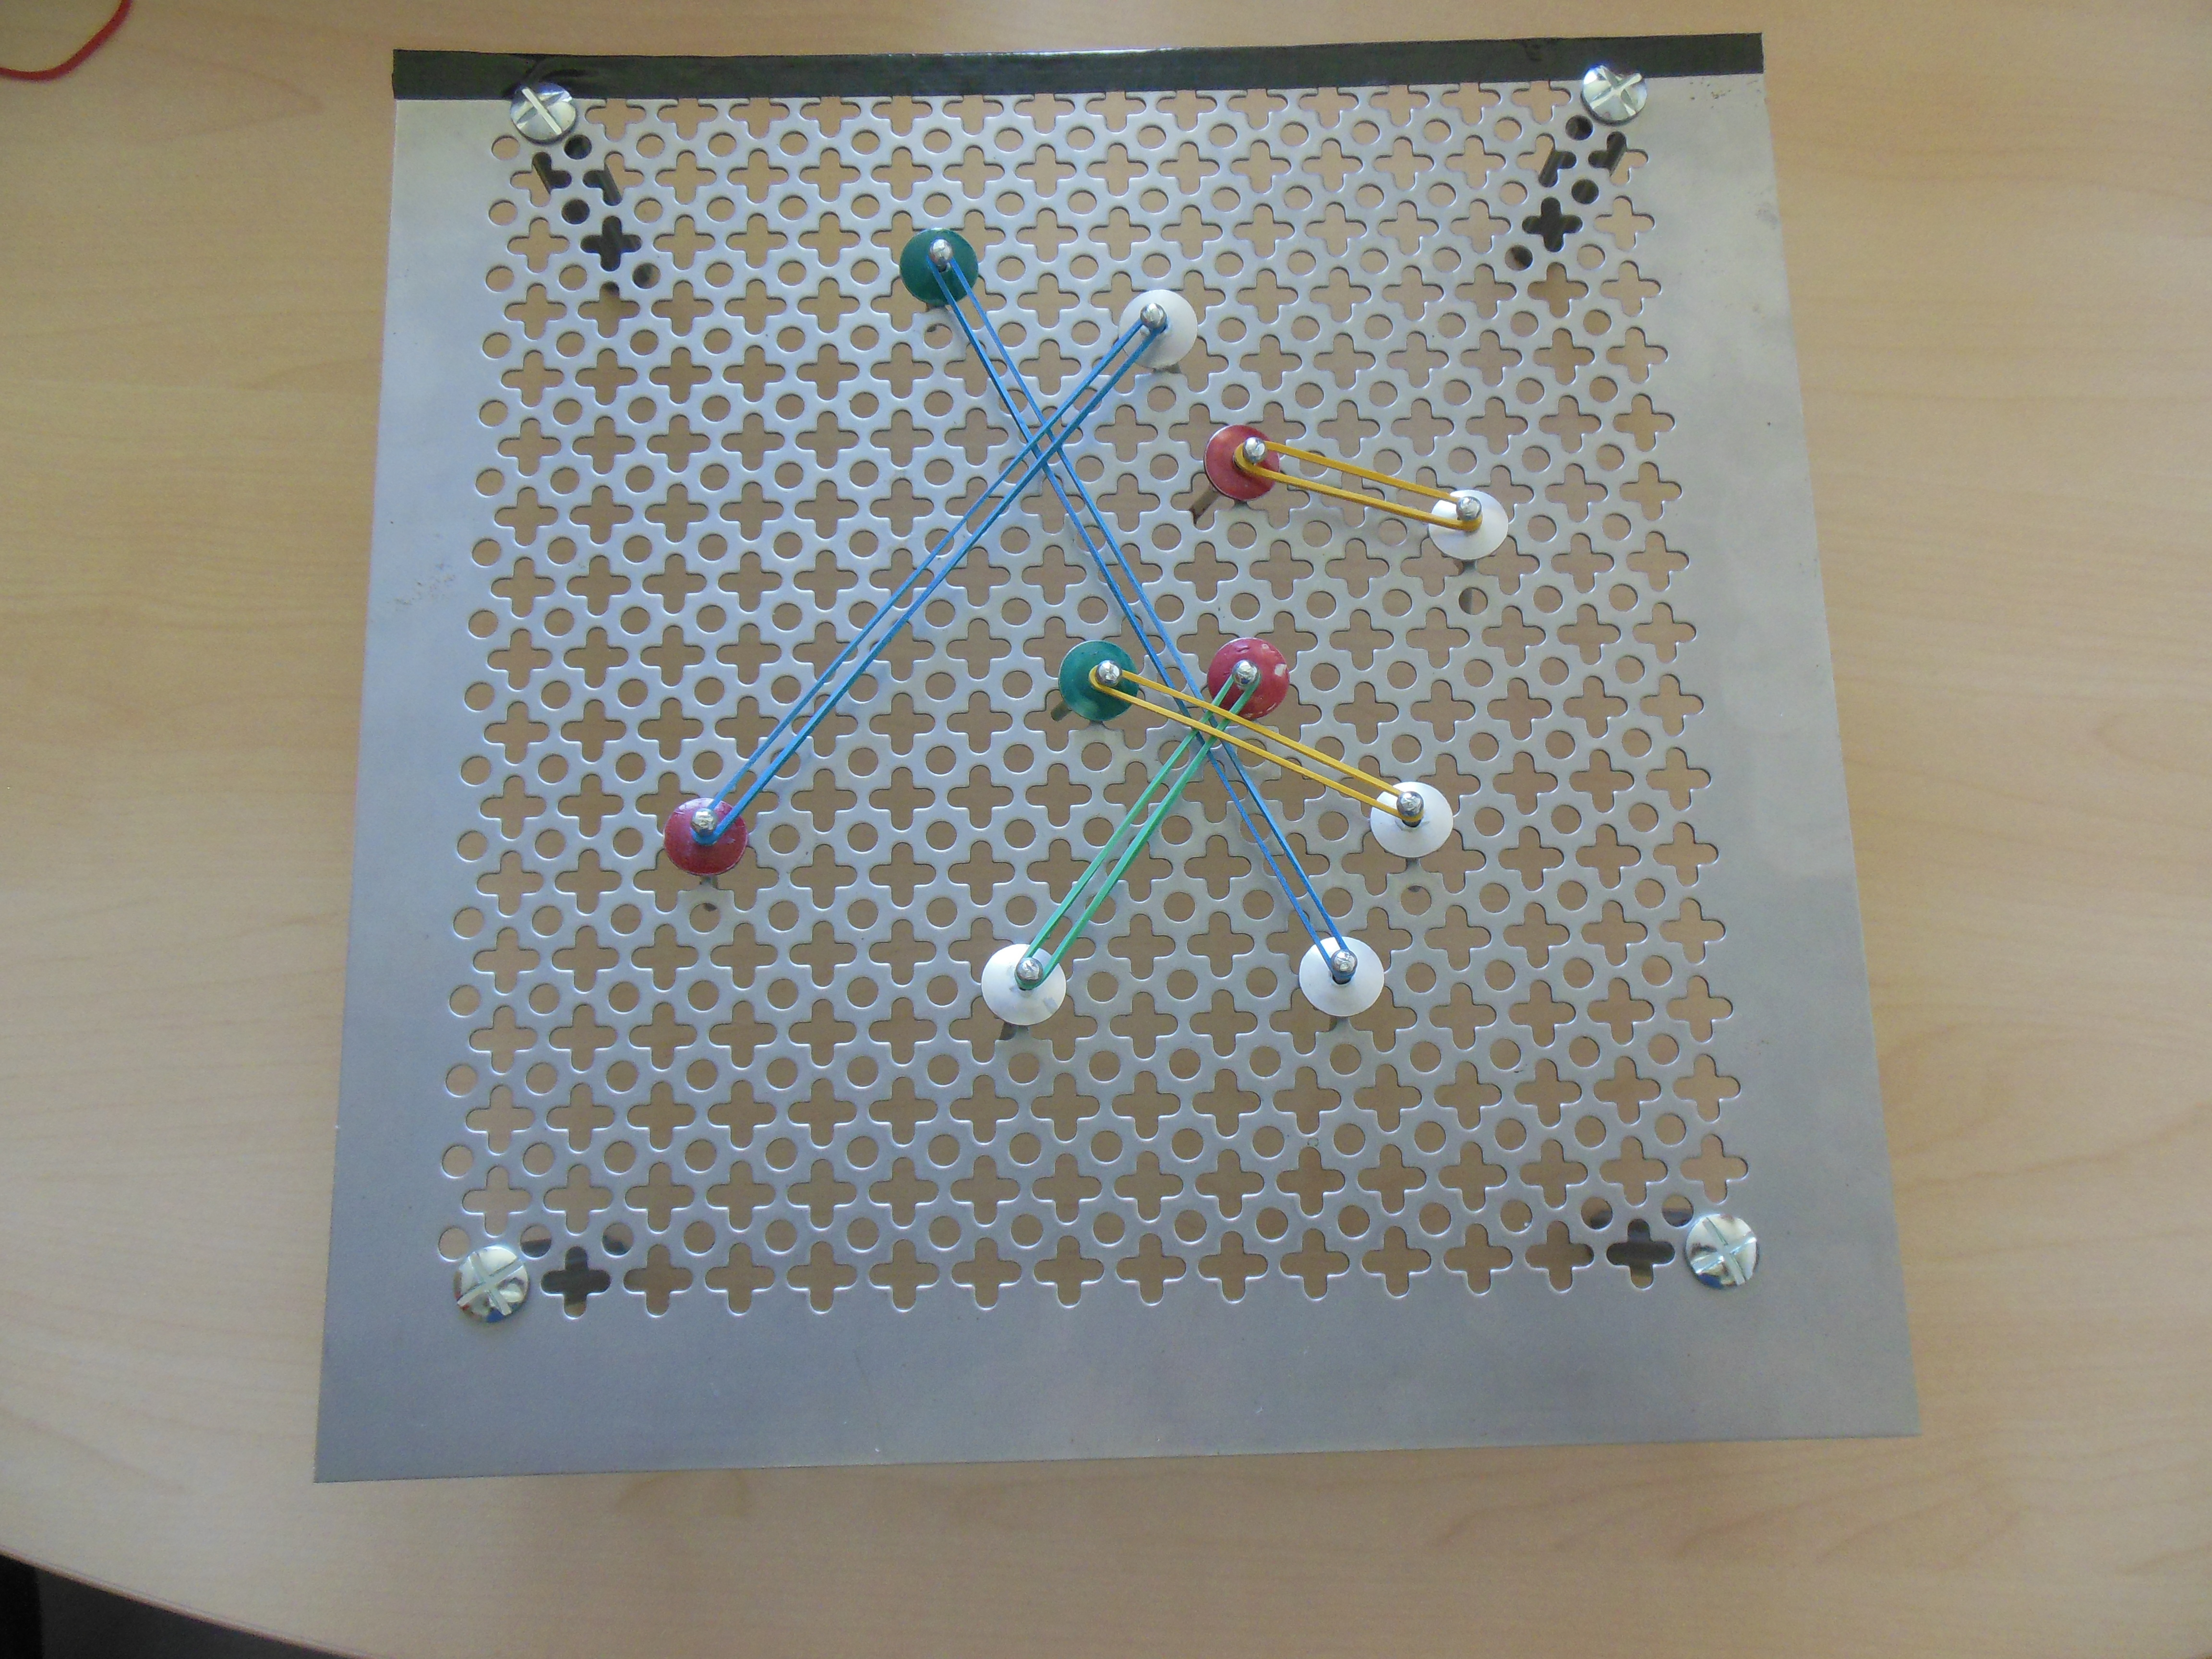
\includegraphics[width=\linewidth]{Photos/Ghosbusters-solution-mauvaise.pdf}
\end{center}
Une mauvaise solution des lasers se croisent.
\end{minipage}\hfill
\begin{minipage}{0.3\linewidth}

\begin{center}
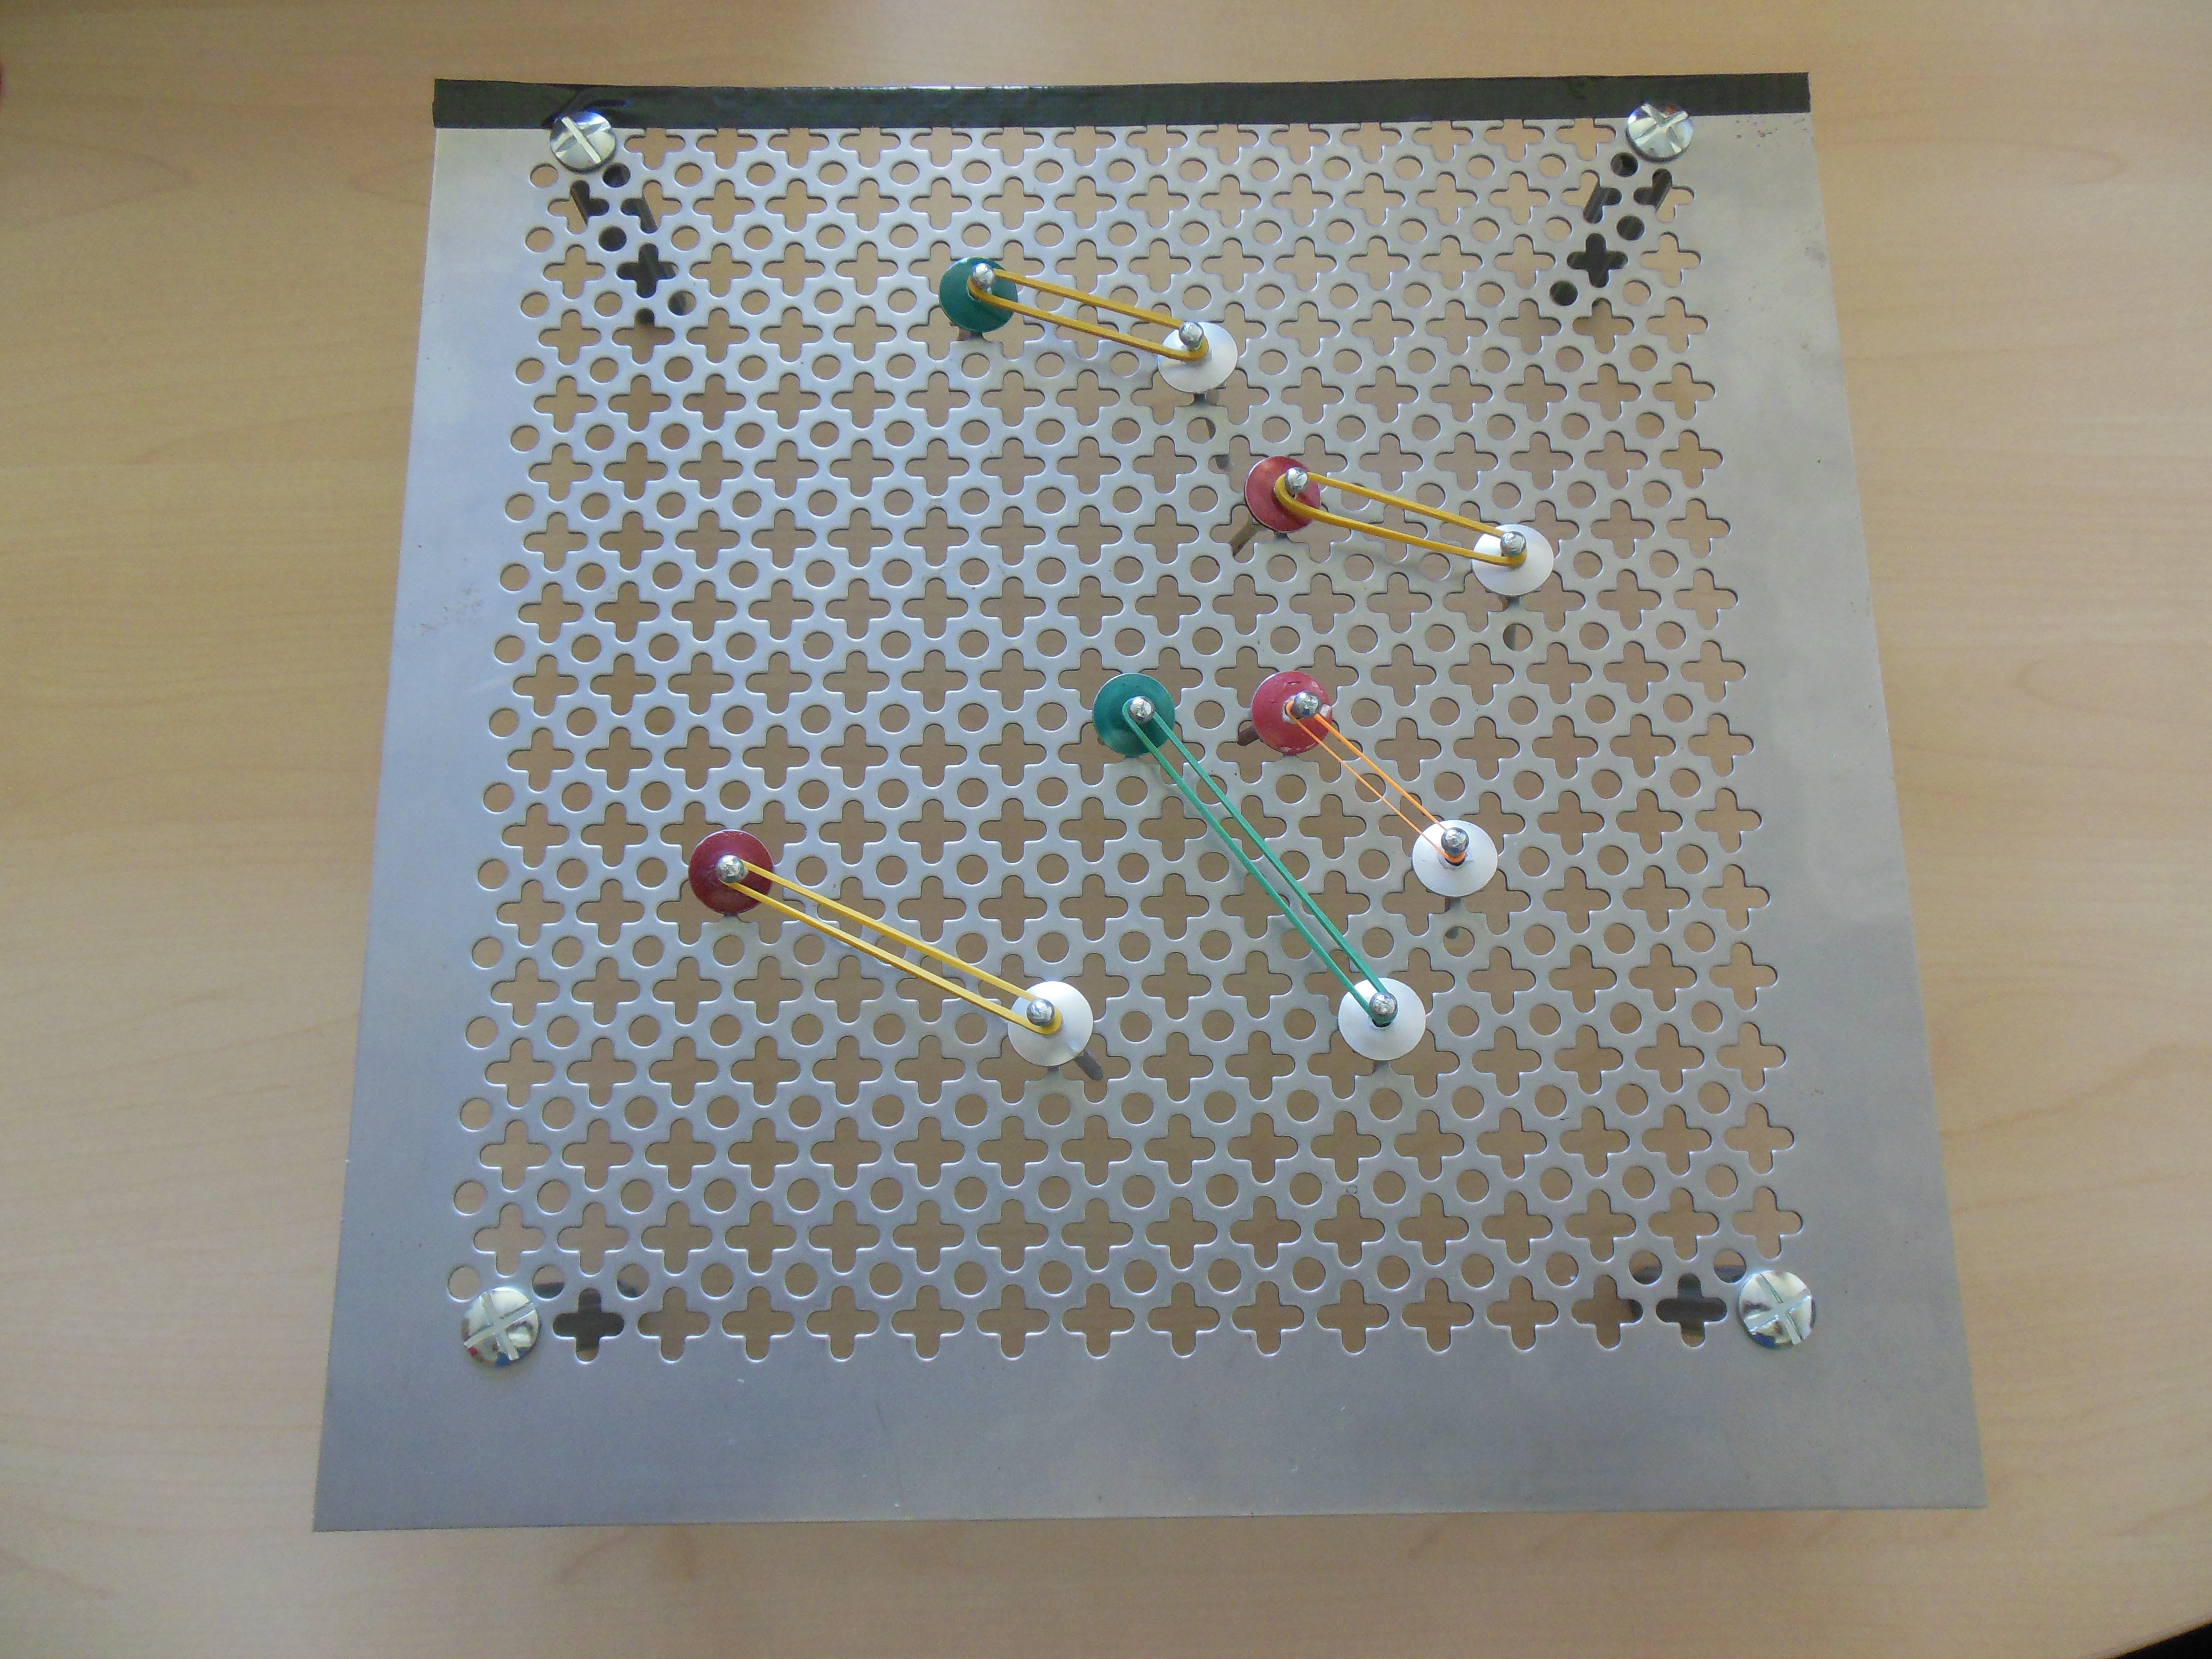
\includegraphics[width=\linewidth]{Photos/Ghostbusters-solution.pdf}
\end{center}
Une bonne solution, le monde ne va pas exploser.
\end{minipage}
\newpage
\subsection*{Existence d'une solution}
Il y a autant de fantômes que de chasseurs. Peut-on toujours trouver une association de chaque  chasseur avec un fantôme sans que les \textit{lasers} s'entrecroisent ?

\begin{Activite}{: on bricole pour dégrossir le problème}
On note $n$ le nombre de chasseurs, $n$ est aussi le nombre de fantômes. Dans un premier temps on peut chercher avec un $n$ significatif ($n=10$ par exemple). 
Avec un peu d'efforts on trouve une solution. Peut-on bouger des fantômes/chasseurs de manière à \textit{empêcher} la solution ? 

On peut restreindre le problème, que se passe-t-il pour des petites valeurs de $n$ ?
On pourra essayer avec $n=1$, $n=2$, $n=3$... 
\end{Activite}
\begin{Indication}{} 
Le problème survient lorsque les points fantômes et les chasseurs sont  alignés. 
\end{Indication}
\subsection*{Heuristiques et contre-exemples}
L'objectif est de trouver une méthode qui permette de résoudre le problème. 

\begin{Activite}{: contre-exemple}
On joue à deux, un propose un algorithme et l'autre cherche un contre-exemple réalisable tel que l'algorithme ne donne pas la solution. 
\end{Activite}
\begin{Indication}{} 
Exemples d'idées d'heuristiques : on choisit le fantôme et le chasseur les plus proches, on joint un couple fantôme/chasseur sur la périphérie (sur l'enveloppe convexe) et on recommence avec le reste, on choisit le fantôme/chasseur les plus bas, ...
\end{Indication}

\subsection*{Diviser pour régner}
À partir des heuristiques, on sent bien que si on réussit à se ramener à un problème plus petit on pourra raisonner par induction. Or le passage de $n$ à $n-1$ parait difficile cf contre-exemples, il faudrait donc découper en \textbf{plusieurs} sous-problèmes. Pour éviter les cas spéciaux on suppose que les points sont en position générale (pas d'alignements), cette hypothèse pourra être affaiblie par la suite.

\begin{Activite}{: un algorithme magistral}
Trouver un couple fantôme/chasseur qui sépare convenablement le nuage des $2(n-1)$ points restants.
\end{Activite}
\begin{Indication}{} 
On choisit un point arbitrairement,  un fantôme par exemple, et on parcourt tous les chasseurs. Pour chaque chasseur on trace la droite entre le chasseur et le fantôme et on compte le nombre de fantômes et de chasseurs en dessous de la droite (au passage définir le "dessous"). Quel point peut-on choisir pour simplifier l'analyse ?
\end{Indication}
\begin{Corrige}{}
\begin{center}
\includegraphics[width=0.6\linewidth]{figures/ghostbusters-separation.fig}
\end{center}


Un point d'ordonnée minimale étant choisi, on suppose que c'est un chasseur (si ce n'est pas le cas échanger le rôle chasseur et fantôme). On trie l'ensemble des autres points ($n$ fantômes et $n-1$ chasseurs) par angle croissant, l'angle étant défini entre le segment et l'axe horizontal orienté. 
On parcourt les points par angle croissant et on calcule le nombre de fantômes/chasseurs dans le secteur angulaire entre la droite et l'axe horizontal  (l'orientation de la droite étant fixée par le segment). 
 
 Le nombre de chasseurs/fantômes va passer de $1,0$ à $n,n$ lorsque tout le demi-plan au-dessus de l'axe horizontal sera balayé. À chaque étapes du parcourt, on ajoute $1$ soit au compte de chasseurs, soit au compte de fantômes. Il y aura donc une première étape pour laquelle le compte de chasseurs et de fantômes sera égal. À cette étape on sera sur un segment associant un chasseur à un fantôme, sinon ce ne serait pas la première fois. 
 
 La droite contenant le segment sépare le nuage de points en 3 parties. Les 2 points (chassuer/fantôme sur la droite), un nombre égal de chasseurs/fantômes dans le secteur angulaire entre la droite et l'axe horizontal  et un nombre égal de  chasseurs/fantômes dans le secteur complémentaire.
 
 Le problème est donc réduit à deux sous-problèmes de même nature dans les 2 secteurs, ces 2 sus-problèmes sont de taille strictement plus petite, on applique donc notre algorithme récursivement sur ces deux sous-problèmes. La droite étant séparatrice, on est certain que les segments construits des deux cotés ne pourront pas s'intersecter, donc leur réunion va former une solution au problème global.
 
 \begin{center}
\includegraphics[width=0.4\linewidth]{figures/ghostbusters-separation-sol.fig}
\end{center}

Le principe utilisé dans cet algorithme est celui du \textbf{diviser pour régner}. On divise le problème en sous-problèmes de même nature mais de taille plus petite, on résout les sous-problèmes et on compose les solutions obtenues pour obtenir la solution au problème initial. Ici la taille des sous-problèmes dépend de la valeur des données et donc sont de taille qui n'est pas connue à l'avance. L'algorithme est très proche de l'algorithme de tri rapide (ou tri par segmentation, \textit{Quicksort}).
Cette approche a été extraite d'un exercice de \citeasnoun{CormenLeisersonRivestStein201006}.
\end{Corrige}
\subsection*{Variant d'itération}
Comme l'objectif est de n'avoir aucun segments qui se croisent, une idée intuitive est, lorsque l'on observe un croisement  de décroiser les segments qui se croisent.

\begin{Activite}{: un algorithme magique} 
Choisir une association chasseurs/fantômes arbitrairement.
Tant qu'il existe des segments qui se croisent, les décroiser. Essayer sur des exemples, essayer de trouver des contre-exemples, observer que décroiser ne diminue pas forcément le nombre de croisements (au fait combien peut-on en avoir ?). Trouver un argument pour prouver que l'algorithme termine en un nombre fini d'étapes. 
\end{Activite}
\begin{Indication}{ géométrique} 
Dans un quadrilatère convexe non dégénéré, les diagonales sont toujours plus grandes que les cotés.
\end{Indication}
\begin{Corrige}{}
Après un choix arbitraire d'affectation, 
l'algorithme consiste en une itération simple : tant qu'il existe un croisement entre 2 segments, décroiser les segments.

Pour prouver la correction de cet algorithme on va trouver un \textit{variant} de l'itération, c'est à dire une fonction des valeurs des variables qui décroisse strictement. Le nombre d'intersections n'est pas un variant de l'itération car il peut augmenter (exemples). Par contre la somme des longueur  des segments diminue. En effet, la somme des longueurs des 2 diagonales d'un quadrilatère non dégénéré est strictement supérieure à la somme des longueurs de 2 cotés opposés. 

La somme des longueurs est donc une fonction strictement décroissante à chaque décroisement. Comme le nombre d'associations est fini, le nombre d'itérations sera fini donc l'algorithme se termine et il n'y a plus de croisements.
\end{Corrige}
\subsection*{Réduction}
Ce problème d'association pourrait-il  simplement être un cas particulier d'un problème général que l'on saurait résoudre ? Pour cela on peut utiliser l'idée de l'algorithme magique en remarquant que la somme des longueurs est minimale en fin d'algorithme.

\begin{Activite}{: un algorithme universel} 
Sur des exemples étudier le minimum obtenu. Est-ce un minimum global ? Et si on avait une méthode pour trouver le minimum global, qu'observerait-on ? Transformer le problème initial en un problème d'optimisation.
\end{Activite}
\begin{Indication}{ algébrique} 
Se donner une représentation algébrique du problème. Quelles sont les variables à utiliser ? Quelles sont les contraintes ?
\end{Indication}
\begin{Corrige}{}
On note $D=((d_{i,j}))$ la matrice $n\times n$ des distances entre chasseurs et fantômes,  $d_{i,j}$ est la distance entre le chasseur $i$ et le fantôme $j$. On cherche alors à minimiser la somme des distances entre les chasseurs et les fantômes. Ce problème est connu sous le nom de \textit{problème d'affectation} ou problème de couplage parfait de poids minimal.

%Le problème est modélisé par un graphe biparti $\mathcal{G}=(\mathcal{C}\cup\mathcal{F},E)$, avec $\mathcal{C}$ l'ensemble des chasseurs, $\mathcal{F}$ l'ensemble des fantômes, et $E=((e_{i,j}))$ l'ensemble des arêtes liant tout chasseur à tout fantôme, l'arête $e_{i,j}$ portant le poids $d_{i,j}$. Un \textbf{couplage} (matching en anglais) est un ensemble d'arêtes tel que les arêtes du couplage n'aient pas de sommet commun.
La méthode (algorithme)  \textit{hongroise} proposé par \citeasnoun{Kuhn1955}, permet de résoudre ce problème par transformations successives de la matrice $D$.


Pour généraliser encore le problème, on peut le modéliser par ce que l'on appelle un \textit{programme linéaire en nombres entiers}.

On note $x_{i,j}$ les variables du problème, $x_{i,j}=1$ si le chasseur $i$ tire sur le fantôme $j$, $x_{i,j}=0$ sinon. On note $X$ la matrice des $x_{i,j}$.

Le problème est donc de minimiser
\[
F(X)= \sum_{i,j} x_{i,j}d_{i,j}, \text{ somme des longueurs de segments;}
\]
sous l'ensemble des contraintes
\[
\sum_{j} x_{i,j} =1 \text{ pour tout chasseur }  i \text{ (un chasseur ne tire que sur un seul fantôme)};
\]
et
\[
\sum_{i} x_{i,j} =1 \text{ pour tout fantôme }  j \text{ (un fantôme n'est  la cible que d'un seul chasseur)}.
\]
Le problème a donc été réduit à une programme linéaire en nombres entiers.

\end{Corrige}

\subsection*{Complexité}
On découvre ainsi plusieurs algorithmes qui permettent de résoudre le même problème, peut-on comparer ces algorithmes, quels seraient les critères de comparaison ? L'écriture, l'efficacité en temps d'exécution ou en mémoire, 

\begin{Activite}{: un algorithme universel} 
Sur des exemples étudier le minimum obtenu. Est-ce un minimum global ? Et si on avait une méthode pour trouver le minimum global, qu'observerait-on ? Transformer le problème initial en un problème d'optimisation.
\end{Activite}
\begin{Indication}{ algébrique} 
Se donner une représentation algébrique du problème. Quelles sont les variables à utiliser ? Quelles sont les contraintes ?
\end{Indication}
\begin{Corrige}{}
On note $D=((d_{i,j}))$ la matrice $n\times n$ des distances entre chasseurs et fantômes,  $d_{i,j}$ est la distance entre le chasseur $i$ et le fantôme $j$. On cherche alors à minimiser la somme des distances entre les chasseurs et les fantômes. Ce problème est connu sous le nom de \textit{problème d'affectation} ou problème de couplage parfait de poids minimal.

%Le problème est modélisé par un graphe biparti $\mathcal{G}=(\mathcal{C}\cup\mathcal{F},E)$, avec $\mathcal{C}$ l'ensemble des chasseurs, $\mathcal{F}$ l'ensemble des fantômes, et $E=((e_{i,j}))$ l'ensemble des arêtes liant tout chasseur à tout fantôme, l'arête $e_{i,j}$ portant le poids $d_{i,j}$. Un \textbf{couplage} (matching en anglais) est un ensemble d'arêtes tel que les arêtes du couplage n'aient pas de sommet commun.
La méthode (algorithme)  \textit{hongroise} proposé par \citeasnoun{Kuhn1955}, permet de résoudre ce problème par transformations successives de la matrice $D$.


Pour généraliser encore le problème, on peut le modéliser par ce que l'on appelle un \textit{programme linéaire en nombres entiers}.

On note $x_{i,j}$ les variables du problème, $x_{i,j}=1$ si le chasseur $i$ tire sur le fantôme $j$, $x_{i,j}=0$ sinon. On note $X$ la matrice des $x_{i,j}$.

Le problème est donc de minimiser
\[
F(X)= \sum_{i,j} x_{i,j}d_{i,j}, \text{ somme des longueurs de segments;}
\]
sous l'ensemble des contraintes
\[
\sum_{j} x_{i,j} =1 \text{ pour tout chasseur }  i \text{ (un chasseur ne tire que sur un seul fantôme)};
\]
et
\[
\sum_{i} x_{i,j} =1 \text{ pour tout fantôme }  j \text{ (un fantôme n'est  la cible que d'un seul chasseur)}.
\]
Le problème a donc été réduit à une programme linéaire en nombres entiers.

\end{Corrige}



\bibliographystyle{agsm}
\bibliography{Ouvrages} 
\label{fin-document}
\end{document}
